\author{Ethan Grant uni: erg2145}
\title{HW05 STAT W4400}
\date{\today}

\documentclass{article}
\usepackage{amsmath}
\usepackage{graphicx}
\begin{document}
	\maketitle
	\begin{enumerate}
		\item
		\begin{enumerate}
			\item 
				\begin{gather*}
					D = {1,2,4,8} \\
					H(x) = -(\sum_{i \epsilon D} p_{i}*log(p_{i})+ L(p_{1},...,p_{d}, \lambda_{0}, \lambda_{1})) \\
					= -(\sum p_{i}*log(p_{i})+ \lambda_{0}*p_{i} + \lambda_{1}*(\sum p_{i}-1) \\
					\frac{dL}{dp_{i}} = \frac{-p_{i}}{p_{i}}-log(p_{i}) +\lambda_{1}=0 \\
					p_{i}* = exp( \lambda_{1}-1)
				\end{gather*}
				The value of $p_{i}$ does not depend on i because $ \lambda_{1}$ does not depend on i and thus $p_{i}$ must have the same value for all i meaning that the maximum entroy solution is the uniform distribution for each distribution
			\item
				To have minimum entropy all the mass for each of the distributions would be at a particular point as described by the dirac. So every distribution equals its dirac (represented by delta) $p(X=i) = \delta_{i} $ for all i in the finite set {1,2,4,8}
			\item
				There are 2 options for each $x_{i}$ in the sequence. Thus there are $2^{n}$ total possible sequences. The result from a tells us that the uniform distribution will have the maximum entropy. From the slides we know that $H(U_{d}) = log_{2}(2^{n}) = n*log_{2}(2^{n}) = n$ where $U_{d}$ is the uniform distribution.
			\item
				We must specify both the start and the transition matrix. Every element in the matrix (which specifices the probability of moving from one value to another) will be the same because it is the uniform distribution. Since there are 2 rows and each column must sum to 1 you know the transition matrix has .5 at each category. Similarly the start must sum to 1 and have equal probability for all elements and since there are 2 elements it is as it is represented below \newline
				P = $\begin{bmatrix}
				.5 & .5 \\
				.5 & .5 
				\end{bmatrix}$ \newline
				$P_{init} = \begin{bmatrix}
				.5 \\
				.5
				\end{bmatrix}$
			\item
				Since we have already found the maximum entropy solution and this solution is not the maximum entropy solution it must have lower entropy than the chain above. 
			\item
				P = $\begin{bmatrix}
				.6 & .3 \\
				.4 & .7 
				\end{bmatrix}$ \newline
				$det ( \begin{bmatrix}
				.6 - \lambda & .3 \\
				.4 & .7 - \lambda
				\end{bmatrix} ) = (.6 - \lambda )(.7 - \lambda) - .12 = 0$ \newline
				$ \lambda_{1} = .3 \lambda_{2} = 1$ \newline
				B/C there is a lambda with a value 1 we know this chain converges \newline
				$E_{1} = ker(\begin{bmatrix}
				-.4 & .3 \\
				.4 & -.3 
				\end{bmatrix} ) = ker( \begin{bmatrix}
				1 & .75 \\
				0 & 0 
				\end{bmatrix} ) = \begin{bmatrix}
				.75 \\
				1
				\end{bmatrix}$ \newline
				normalize this eigenvector
				$ \frac{\begin{bmatrix}
					.75 \\
					1
					\end{bmatrix}}{\sqrt{.75^{2}+1}} = \begin{bmatrix}
				.6 \\
				.8
				\end{bmatrix} $ \newline
				Want the columns to sum to 1 so need to do that while maintaining the ratio of $\begin{bmatrix}
					.6 \\
					.8
				\end{bmatrix}$ note .6 = 3*.2 and .8 = 4*.2 thus can transform matrix to: \newline
				$p_{eq} = \begin{bmatrix}
				\frac{3}{7} \\
				\frac{4}{7}
				\end{bmatrix}$
			\item 
				By definition $lim_{n-> \infty}p_{n} = p^{n}*p_{eq}=p_{eq}$ so $lim_{n-> \infty}(Pr(x=1)) = 4/7$ and $lim_{n-> \infty}(Pr(x=0)) = 3/7$
			\item
				Important info: $H[X_{i}|H_{i-1}]=H[X_{2}|H_{1}]$ based on the Markov properties since you are starting from the equilibirum vector. Thus you only need to calculate $H[X_{2}|H_{1}]$ which will occur n-1 times and $H[X_{1}]$ to deterimine the entropy of the whole chain \newline
				Also note all logs are base 2 as is customary: \newline
				$H(X_{1}) = -4/7*log(4/7)-3/7*log(3/7) = .9852$ \newline
				Some probabilities that will be used in the following calculation where P(x,y) = $P(x_{2}, x_{1})$:  \newline
				$P(1, 0 ) = .3*3/7$ \newline
				$P(1, 1 ) = .7*4/7$ \newline
				$P(0, 0 ) = .6*3/7$ \newline 
				$P(0, 1 ) = .4*4/7$ \newline
				$H[X_{2}|H_{1}] = -(.4*4/7*log(.7) + .3*4/7*log(.3)+.6*3/7*log(.6)+.4*3/7*log(.4) = .91972$ \newline
				Total Entropy = $.9852 + (n-1)*.91972$
		\end{enumerate}
		\item
		\begin{enumerate}
			\item Graph: $e^{0} = 1 e^{-1} = 1/e ... e^{-4} = 1/(e^{4})$ \newline
				 \begin{minipage}{\linewidth}
				 	\centering
						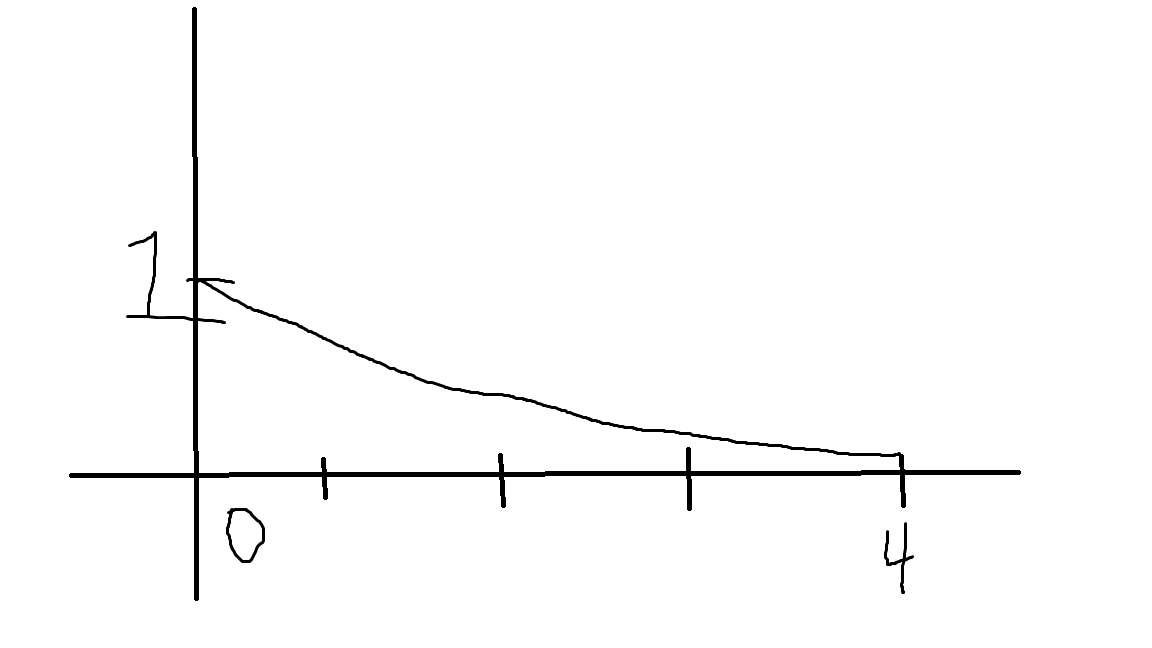
\includegraphics[scale=.5]{graph}
				 \end{minipage}		
			\item 
				There is no visual representation of the likelihood of an individual point on a pdf. the likelihood is the product of the exponential at the points 1 , 2, 4 
			\item
				The higher rate would decrease the likelihood for the toy data set. Observe that p(1,2) = 2/$e^{2}$ < 1/e , p(2,2)=2/$e^{4}$ < 1/$e^{2}$ , p(4,2)=4/$e^{8}$ < 1/$e^{4}$. Since the individual likelihoods are all smaller their product is smaller as well and since the product is the definition of likelihood the likelihood declines
			\item 
				\begin{gather*}
					 q(\theta| x_{1} ... x_{n})= \frac{\Pi^{n}( \theta * e^{-\theta * x_{i}})*\frac{\theta^{\alpha_{0}-1}*\beta^{\alpha_{0}}*e^{-\beta_{0}*\theta}}{\Gamma(\alpha_{0})}}{p(x_{1},...,x_{n})} \\
					 aside: c = \frac{1}{\Gamma(\alpha_{0})*p(x_{1} ... x_{n})} \\
					 = c*\theta^{n}*e^{-\theta*\sum(x_{i})}*\theta^{\alpha_{0}-1}*\beta^{\alpha_{0}}*e^{-\beta_{0}*\theta} \\
					 =c*\theta^{\alpha_{0}+n-1}*e^{-\theta*(\sum(x_{i})+\beta_{0}} \\
					 = gamma(\theta, \alpha_{0}+n, \sum x_{i}+\beta_{0})
				\end{gather*}
			\item
				You can define the value from 1 to n (using all data points) easily based on the definitions provided: 
				\begin{gather*}
					\Pi(\theta | x_{1},...,x_{n}) = \frac{\Pi_{i}^{n}p(x_{i}|\theta)*q(\theta)}{\Pi_{1}^{n}p(x_{i})} 
				\end{gather*}
				You can then seperate out the nth calculation because you are just multiplying leaving you with the posterior for n-1 calcuations times the nth observation
				\begin{gather*}
					\Pi(\theta | x_{1},...,x_{n}) = \frac{p(x_{n}|\theta)}{p(x_{n})} \frac{\Pi_{i}^{n-1}p(x_{i}|\theta)*q(\theta)}{\Pi_{1}^{n-1}p(x_{i})} \\
				\end{gather*}
				thus we can see that prior can now be defined as:
				\begin{gather*}
					q(\theta) = \Pi(\theta|x_{1},...,x_{n-1}) = \frac{\Pi_{i}^{n-1}p(x_{i}|\theta)*q(\theta)}{\Pi_{1}^{n-1}p(x_{i})}
				\end{gather*}
			\item
				This is based on the answer to problem 2.d. The sum of new x's is merely summing $x_{n}$ because it is the only new point and thus all that is added to $beta_{n-1}$ and there is only 1 to add to $\alpha_{n-1}$. 
				\begin{gather*}
					g(\theta|x_{n}) = Gamma(\theta, \alpha_{n-1}+1, \beta_{n-1}+x_{n})
				\end{gather*}
			\item
				As n increases the variance will decrease and the function will have a higher peak that is centered more tightly around the value of theta 
				The gray line with the highest peak has an n =256 \newline
				the purple line has n = 16 \newline
				the blue line has n = 8 \newline
				the black line has n =4
				\begin{minipage}{\linewidth}
					\centering
					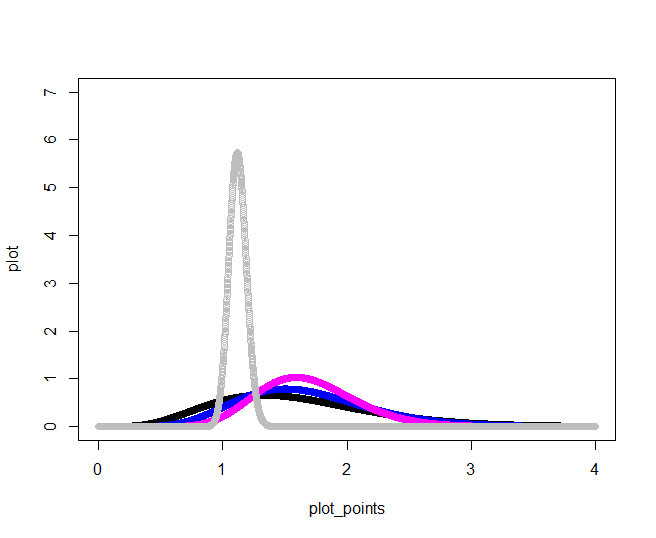
\includegraphics[scale=.5]{gamma}
				\end{minipage}	
			
		\end{enumerate}
	\end{enumerate}
\end{document}